\documentclass{article}\usepackage[]{graphicx}\usepackage[]{color}
%% maxwidth is the original width if it is less than linewidth
%% otherwise use linewidth (to make sure the graphics do not exceed the margin)
\makeatletter
\def\maxwidth{ %
  \ifdim\Gin@nat@width>\linewidth
    \linewidth
  \else
    \Gin@nat@width
  \fi
}
\makeatother

\definecolor{fgcolor}{rgb}{0.345, 0.345, 0.345}
\newcommand{\hlnum}[1]{\textcolor[rgb]{0.686,0.059,0.569}{#1}}%
\newcommand{\hlstr}[1]{\textcolor[rgb]{0.192,0.494,0.8}{#1}}%
\newcommand{\hlcom}[1]{\textcolor[rgb]{0.678,0.584,0.686}{\textit{#1}}}%
\newcommand{\hlopt}[1]{\textcolor[rgb]{0,0,0}{#1}}%
\newcommand{\hlstd}[1]{\textcolor[rgb]{0.345,0.345,0.345}{#1}}%
\newcommand{\hlkwa}[1]{\textcolor[rgb]{0.161,0.373,0.58}{\textbf{#1}}}%
\newcommand{\hlkwb}[1]{\textcolor[rgb]{0.69,0.353,0.396}{#1}}%
\newcommand{\hlkwc}[1]{\textcolor[rgb]{0.333,0.667,0.333}{#1}}%
\newcommand{\hlkwd}[1]{\textcolor[rgb]{0.737,0.353,0.396}{\textbf{#1}}}%

\usepackage{framed}
\makeatletter
\newenvironment{kframe}{%
 \def\at@end@of@kframe{}%
 \ifinner\ifhmode%
  \def\at@end@of@kframe{\end{minipage}}%
  \begin{minipage}{\columnwidth}%
 \fi\fi%
 \def\FrameCommand##1{\hskip\@totalleftmargin \hskip-\fboxsep
 \colorbox{shadecolor}{##1}\hskip-\fboxsep
     % There is no \\@totalrightmargin, so:
     \hskip-\linewidth \hskip-\@totalleftmargin \hskip\columnwidth}%
 \MakeFramed {\advance\hsize-\width
   \@totalleftmargin\z@ \linewidth\hsize
   \@setminipage}}%
 {\par\unskip\endMakeFramed%
 \at@end@of@kframe}
\makeatother

\definecolor{shadecolor}{rgb}{.97, .97, .97}
\definecolor{messagecolor}{rgb}{0, 0, 0}
\definecolor{warningcolor}{rgb}{1, 0, 1}
\definecolor{errorcolor}{rgb}{1, 0, 0}
\newenvironment{knitrout}{}{} % an empty environment to be redefined in TeX

\usepackage{alltt}
\usepackage[margin=1in]{geometry}
\usepackage[colorlinks=true]{hyperref}
\usepackage{harvard}
\usepackage{subcaption}
\usepackage{booktabs}
\usepackage{fancyvrb}

\title{Web Scraping With \texttt{R}}
\author{William Marble\thanks{Prepared for the political science/international relations Summer Research College at Stanford. Vincent Bauer's \href{http://stanford.edu/~vbauer/VAMScrapingSlides.html}{excellent slides} on web scraping were very helpful in preparing this tutorial (and teaching me web scraping in \texttt{R} in the first place). The code used in this tutorial can be downloaded at \href{www.stanford.edu/~wpmarble/webscraping_tutorial/code.R}{{www.stanford.edu/\textasciitilde wpmarble/webscraping\_tutorial/code.R}}. Feel free to email me with questions or comments at \href{mailto:wpmarble@stanford.edu}{wpmarble@stanford.edu}.}}
\date{August 11, 2016}
\IfFileExists{upquote.sty}{\usepackage{upquote}}{}
\begin{document}

\maketitle

There is a wealth of valuable information that is publicly available online, but seems to be locked away in web pages that are not amenable to data analysis. While many organizations make their data easily available for researchers, this practice is still the exception rather than the rule -- and, oftentimes, the data we seek may not be centralized or the creators may not have intended to create a database. But researchers are increasingly turning to these useful data sources.

For example, \citeasnoun{Grimmer2013b} analyzes press releases from members of Congress to study how representatives communicate to their constituents. Similarly, \citeasnoun{Nielsen2015} use European Union press releases to measure whether treaty ratification leads to praise from the international community. In both cases, these documents were available online, but they were not centralized and their authors did not intend to create a database of press releases for researchers to analyze. Nonetheless, they represent valuable data for important social science questions --- if we have a way to put them into a more usable format.

Fortunately, there are many tools available for translating unruly HTML into more structured databases. The goal of this tutorial is to provide an introduction to the philosophy and basic implementation of ``web scraping'' using the open-source statistical programming language \texttt{R}.\footnote{Python is another programming language that has excellent capabilities for web scraping --- particularly with the \texttt{BeautifulSoup} package. However, I focus on \texttt{R} because more social scientists tend to be familiar with it than with Python.} I think the best way to learn webscraping is by doing it, so after a brief overview of the tools, most of this document will be devoted to working through examples.

\section{High-Level Overview: the Process of Webscraping}

There are essentially six steps to extracting text-based data from a website:
\begin{enumerate}
  \item Identify information on the internet that you want to use. 
  \item If this information is stored on more than one web page, figure out how to automatically navigate to the web pages. In the best case scenario, you will have a directory page or the URL will have a consistent pattern that you can recreate --- e.g., \texttt{www.somewebsite.com/year/month/day.html}.\label{step2}
  \item Locate the features on the website that flag the information you want to extract. This means looking at the underlying HTML to find the elements you want and/or identifying some sort of pattern in the website's text that you can exploit.\label{step3}
  \item Write a script to extract, format, and save the information you want using the flags you identified.\label{step4}
  \item Loop through all the websites from step~\ref{step2}, applying the script to each of them.
  \item Do some awesome analysis on your newly unlocked data!\label{laststep}
\end{enumerate}
This tutorial will focus on steps~\ref{step3} and~\ref{step4}, which are the most difficult part of webscraping. 

There is also another, simpler way to do webscraping that I'll show an example of: namely, using \textbf{A}pplication \textbf{P}rogramming \textbf{I}nterfaces (APIs) that some websites make available. APIs basically give you a simple way to query a database and return the data you ask for in a nice format (usually JSON or XML). APIs are great, but aren't usually available, so I don't emphasize them here.

\section{Basics of HTML and Identifying the Info We Want}

Hypertext Markup Language --- or HTML --- is a standardized system for writing web pages. Its structure is fairly simple, and understanding its basics is important for successful web scraping. 

This is basically what a website looks like under the hood:\footnote{To see what this webpage looks like in a browser, go to \href{http://stanford.edu/~wpmarble/webscraping_tutorial/html/silly_webpage.html}{this link}.}

\begin{knitrout}
\definecolor{shadecolor}{rgb}{0.969, 0.969, 0.969}\color{fgcolor}\begin{kframe}
\begin{alltt}
<!DOCTYPE html> 
<html> 
  
  <head>
    <title>This is the title of the webpage</title>
  </head>
  
  <body>
    <h1>This is a heading</h1>  
    <p class=\hlstr{"notThisOne"}>This is a paragraph</p>  
    <p class=\hlstr{"thisOne"}>This is another paragraph with a different class!</p>  
    
    <div id=\hlstr{"myDivID"}> 
      <p class=\hlstr{"divGraf"}> 
        This is a paragraph inside a division, along with a 
        <a href=\hlstr{"http://stanford.edu"}>a link</a>.
      </p> 
    </div>
  </body> 

</html>
\end{alltt}
\end{kframe}
\end{knitrout}

\begin{figure}
  \centering
  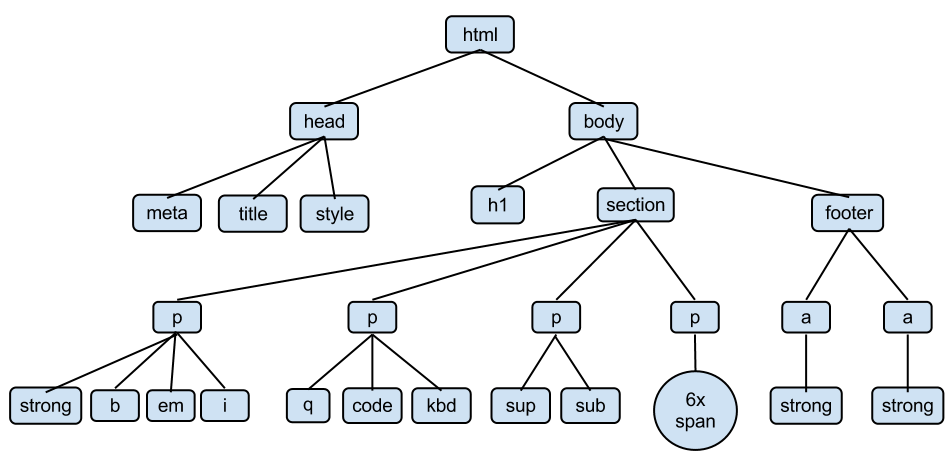
\includegraphics[width=.75\textwidth]{HTMLDOMTree.png}
  \caption{HTML document tree. Source: \url{http://www.openbookproject.net/tutorials/getdown/css/images/lesson4/HTMLDOMTree.png}}\label{fig:htmltree}
\end{figure}

Figure~\ref{fig:htmltree} also provides a visual representation of an HTML tree. 

There are several things to note about this structure. First, elements are always surrounded by code that tells web browsers what they are. These tags are opened with triangular brackets \verb!<tag>! and closed with a slash inside more triangular brackets \verb!</tag>!. Second, these tags often have additional information, such as information about the \texttt{class}. Third, these elements are always nested inside other elements. Together, we can use these features to extract the data we want. 

It's easy to see the underlying HTML for any webpage: in Chrome, click View $\rightarrow$ Developer $\rightarrow$ View Source. This is the first thing you should do when you want to extract data from a webpage. There is also an excellent Chrome add-on called \href{http://selectorgadget.com/}{SelectorGadget} that allows you to point-and-click the parts of the website that you want to extract. It will automatically tell you what the underlying tags are, and you can copy-paste that into your script. 

\section{Tools for Webscraping}

\subsection{\texttt{rvest}}
How can you select elements of a website in \texttt{R}? The \texttt{rvest} package is the workhorse toolkit. The workflow typically is as follows:\footnote{More information can be found on the GitHub page for \href{https://github.com/hadley/rvest}{rvest}.}
\begin{enumerate}
  \item Read a webpage using the function \verb!read_html()!. This function will download the HTML and store it so that \texttt{rvest} can navigate it. 
  \item Select the elements you want using the function \verb!html_nodes()!. This function will take an HTML object (from \verb!read_html!) along with a CSS or Xpath selector (e.g., \verb!p! or \verb!span!) and save all the elements that match the selector. This is where SelectorGadget can be helpful. 
  \item Extract components of the nodes you've selected using functions like \verb!html_tag()! (the name of the tag), \verb!html_text()! (all text inside the tag), \verb!html_attr()! (contents of a single attribute) and \verb!html_attrs()! (all attributes). 
\end{enumerate}

The \texttt{rvest} package also has other features that are more advanced --- such as the ability to fill out forms on websites and navigate websites as if you were using a browser. 

\subsection{Regular Expressions}
Oftentimes you'll see a pattern in text that you'll want to exploit. For instance, a new variable might always follow a colon that comes after  a single word in a new line. Regular expressions (or regex) is a language to precisely define those patterns. They're pretty crucial for webscraping and text analysis. Explaining regex is beyond the scope of this tutorial but I posted a good cheatsheet from AddedBytes.com \href{http://stanford.edu/~wpmarble/webscraping_tutorial/regex_cheatsheet.pdf}{at this link}. In \texttt{R}, some regex commands you might need to use:
\begin{itemize}
  \item \verb!grep(pattern, string)! \\
  This command takes a string vector and returns a vector of the indices of the string that match the pattern
\begin{knitrout}
\definecolor{shadecolor}{rgb}{0.969, 0.969, 0.969}\color{fgcolor}\begin{kframe}
\begin{alltt}
\hlstd{string} \hlkwb{=} \hlkwd{c}\hlstd{(}\hlstr{"this is"}\hlstd{,} \hlstr{"a string"}\hlstd{,} \hlstr{"vector"}\hlstd{,} \hlstr{"this"}\hlstd{)}
\hlkwd{grep}\hlstd{(}\hlstr{"this"}\hlstd{, string)}
\end{alltt}
\begin{verbatim}
## [1] 1 4
\end{verbatim}
\end{kframe}
\end{knitrout}
  
  \item \verb!grepl(pattern, string)! \\
  This command takes a string vector with length \texttt{n} as an input and returns a logical vector of length \texttt{n} that says whether the string matches the pattern. Example:
\begin{knitrout}
\definecolor{shadecolor}{rgb}{0.969, 0.969, 0.969}\color{fgcolor}\begin{kframe}
\begin{alltt}
\hlkwd{grepl}\hlstd{(}\hlstr{"this"}\hlstd{, string)}
\end{alltt}
\begin{verbatim}
## [1]  TRUE FALSE FALSE  TRUE
\end{verbatim}
\end{kframe}
\end{knitrout}
  \item \verb!gsub(pattern, replacement, string)! \\
  This command finds all the instances of \texttt{pattern} in \texttt{string} and replaces it with \texttt{replacement}. Example:
\begin{knitrout}
\definecolor{shadecolor}{rgb}{0.969, 0.969, 0.969}\color{fgcolor}\begin{kframe}
\begin{alltt}
\hlkwd{gsub}\hlstd{(}\hlkwc{pattern}\hlstd{=}\hlstr{"is"}\hlstd{,} \hlkwc{replacement}\hlstd{=}\hlstr{"WTF"}\hlstd{, string)}
\end{alltt}
\begin{verbatim}
## [1] "thWTF WTF" "a string"  "vector"    "thWTF"
\end{verbatim}
\end{kframe}
\end{knitrout}
  
\end{itemize}

\section{Simple Example of Webscraping}

Let's see what that fake website above looks like in \texttt{rvest}. I'll first read in the HTML, then I'll select all paragraphs, then select elements with class ``thisOne,'' then select elements with the ID ``myDivID.'' Finally, I'll extract some text and the link.

\begin{knitrout}
\definecolor{shadecolor}{rgb}{0.969, 0.969, 0.969}\color{fgcolor}\begin{kframe}
\begin{alltt}
\hlcom{## First, load required packages (or install if they're not already)}
\hlstd{pkgs} \hlkwb{=} \hlkwd{c}\hlstd{(}\hlstr{"rvest"}\hlstd{,} \hlstr{"magrittr"}\hlstd{,} \hlstr{"httr"}\hlstd{,} \hlstr{"stringr"}\hlstd{)}
\hlkwa{for} \hlstd{(pkg} \hlkwa{in} \hlstd{pkgs)\{}
  \hlkwa{if} \hlstd{(}\hlopt{!}\hlkwd{require}\hlstd{(pkg,} \hlkwc{character.only} \hlstd{= T))\{}
    \hlkwd{install.packages}\hlstd{(pkg)}
    \hlkwd{library}\hlstd{(pkg)}
  \hlstd{\}}
\hlstd{\}}
\end{alltt}
\end{kframe}
\end{knitrout}
\begin{knitrout}
\definecolor{shadecolor}{rgb}{0.969, 0.969, 0.969}\color{fgcolor}\begin{kframe}
\begin{alltt}
\hlcom{## Read my example html with read_html()}
\hlstd{silly_webpage} \hlkwb{=} \hlkwd{read_html}\hlstd{(}\hlstr{"http://stanford.edu/~wpmarble/webscraping_tutorial/html/silly_webpage.html"}\hlstd{)}

\hlcom{# get paragraphs (css selector "p")}
\hlstd{my_paragraphs} \hlkwb{=} \hlkwd{html_nodes}\hlstd{(silly_webpage,} \hlstr{"p"}\hlstd{)}
\hlstd{my_paragraphs}
\end{alltt}
\begin{verbatim}
## {xml_nodeset (3)}
## [1] <p class="notThisOne">This is a paragraph</p>
## [2] <p class="thisOne">This is another paragraph with a different class! ...
## [3] <p class="divGraf"> \n        This is a paragraph inside a division, ...
\end{verbatim}
\begin{alltt}
\hlcom{# get elements with class "thisOne" -- use a period to denote class}
\hlstd{thisOne_elements} \hlkwb{=} \hlkwd{html_nodes}\hlstd{(silly_webpage,} \hlstr{".thisOne"}\hlstd{)}
\hlstd{thisOne_elements}
\end{alltt}
\begin{verbatim}
## {xml_nodeset (1)}
## [1] <p class="thisOne">This is another paragraph with a different class! ...
\end{verbatim}
\begin{alltt}
\hlcom{# get elements with id "myDivID" -- use a hashtag to denote id}
\hlstd{myDivID_elements} \hlkwb{=} \hlkwd{html_nodes}\hlstd{(silly_webpage,} \hlstr{"#myDivID"}\hlstd{)}
\hlstd{myDivID_elements}
\end{alltt}
\begin{verbatim}
## {xml_nodeset (1)}
## [1] <div id="myDivID"> \n      <p class="divGraf"> \n        This is a p ...
\end{verbatim}
\begin{alltt}
\hlcom{# extract text from myDivID_elements}
\hlstd{myDivID_text} \hlkwb{=} \hlkwd{html_text}\hlstd{(myDivID_elements)}
\hlstd{myDivID_text}
\end{alltt}
\begin{verbatim}
## [1] " \n       \n        This is a paragraph inside a division, along with a \n        a link.\n       \n    "
\end{verbatim}
\begin{alltt}
\hlcom{# extract links from myDivID_elements. first i extract all the "a" nodes (as in a href="website.com")}
\hlcom{# and then extract the "href" attribute from those nodes}
\hlstd{myDivID_link} \hlkwb{=} \hlkwd{html_nodes}\hlstd{(myDivID_elements,} \hlstr{"a"}\hlstd{)} \hlopt \hlkwd{html_attr}\hlstd{(}\hlstr{"href"}\hlstd{)}
\hlstd{myDivID_link}
\end{alltt}
\begin{verbatim}
## [1] "http://stanford.edu"
\end{verbatim}
\end{kframe}
\end{knitrout}

Here, I used CSS selectors (class and ID) to extract nodes from the HTML. One thing to note is that to select classes, you put a period before the name of the class --- \verb!html_nodes(silly_webpage, ".thisOne")!. To select ID's, put a hashtag in front of the ID you want --- \verb!html_nodes(silly_webpage, "#myDivID")!. 

\section{More Difficult Example}

\begin{figure}[!t]
  \centering
  \begin{subfigure}[b]{.5\textwidth}
    \centering
    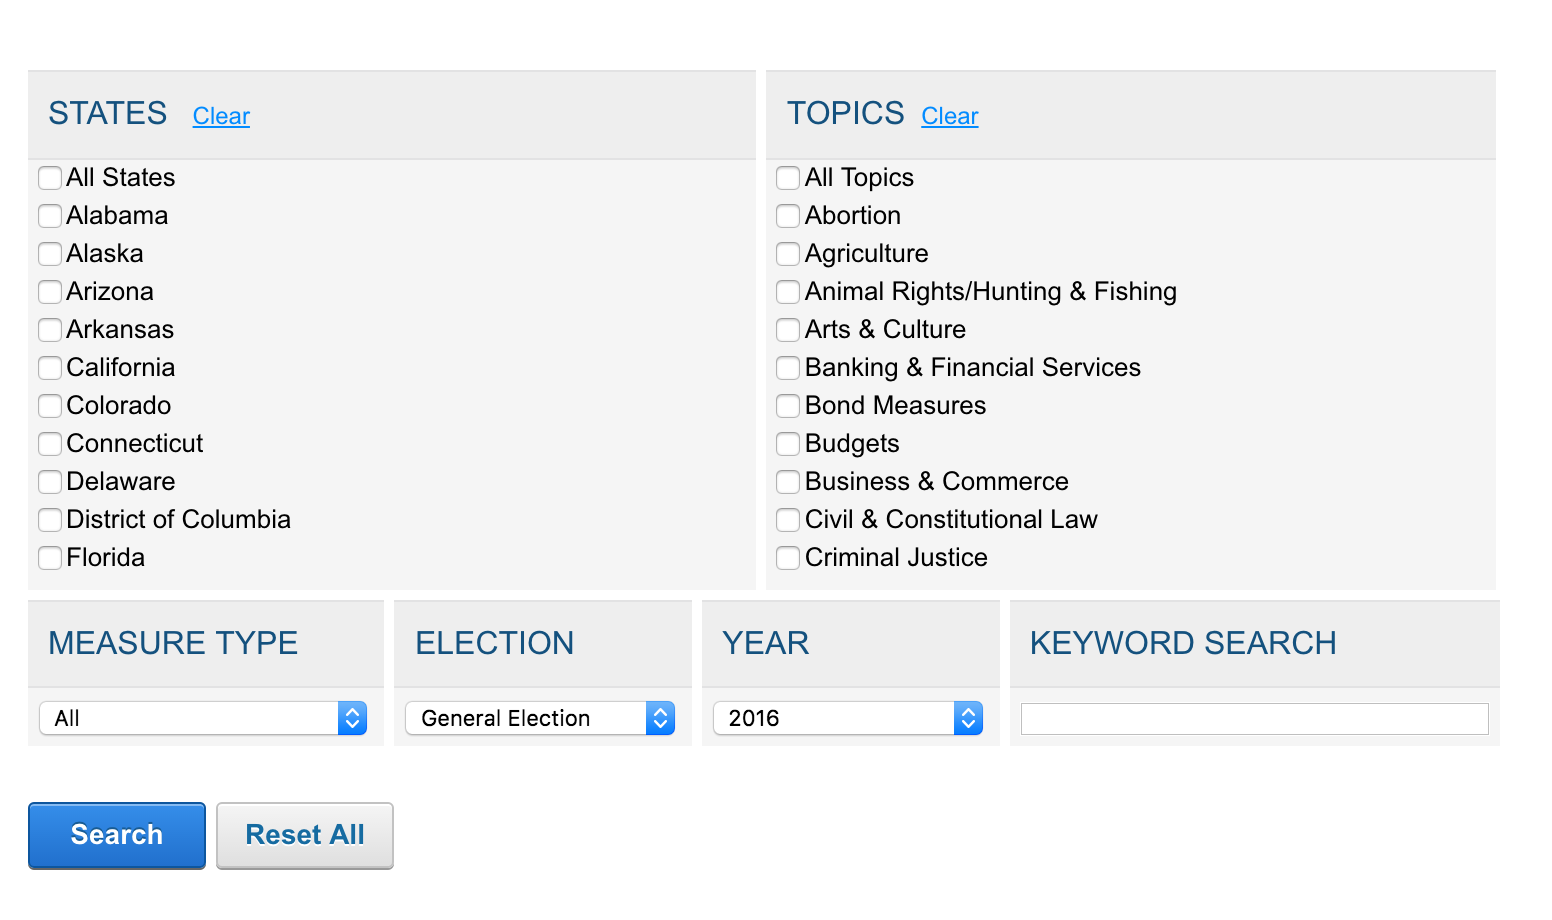
\includegraphics[width=.9\textwidth]{ncsl_database.png}\caption{Search interface}
  \end{subfigure}%
  \begin{subfigure}[b]{.5\textwidth}
    \centering
    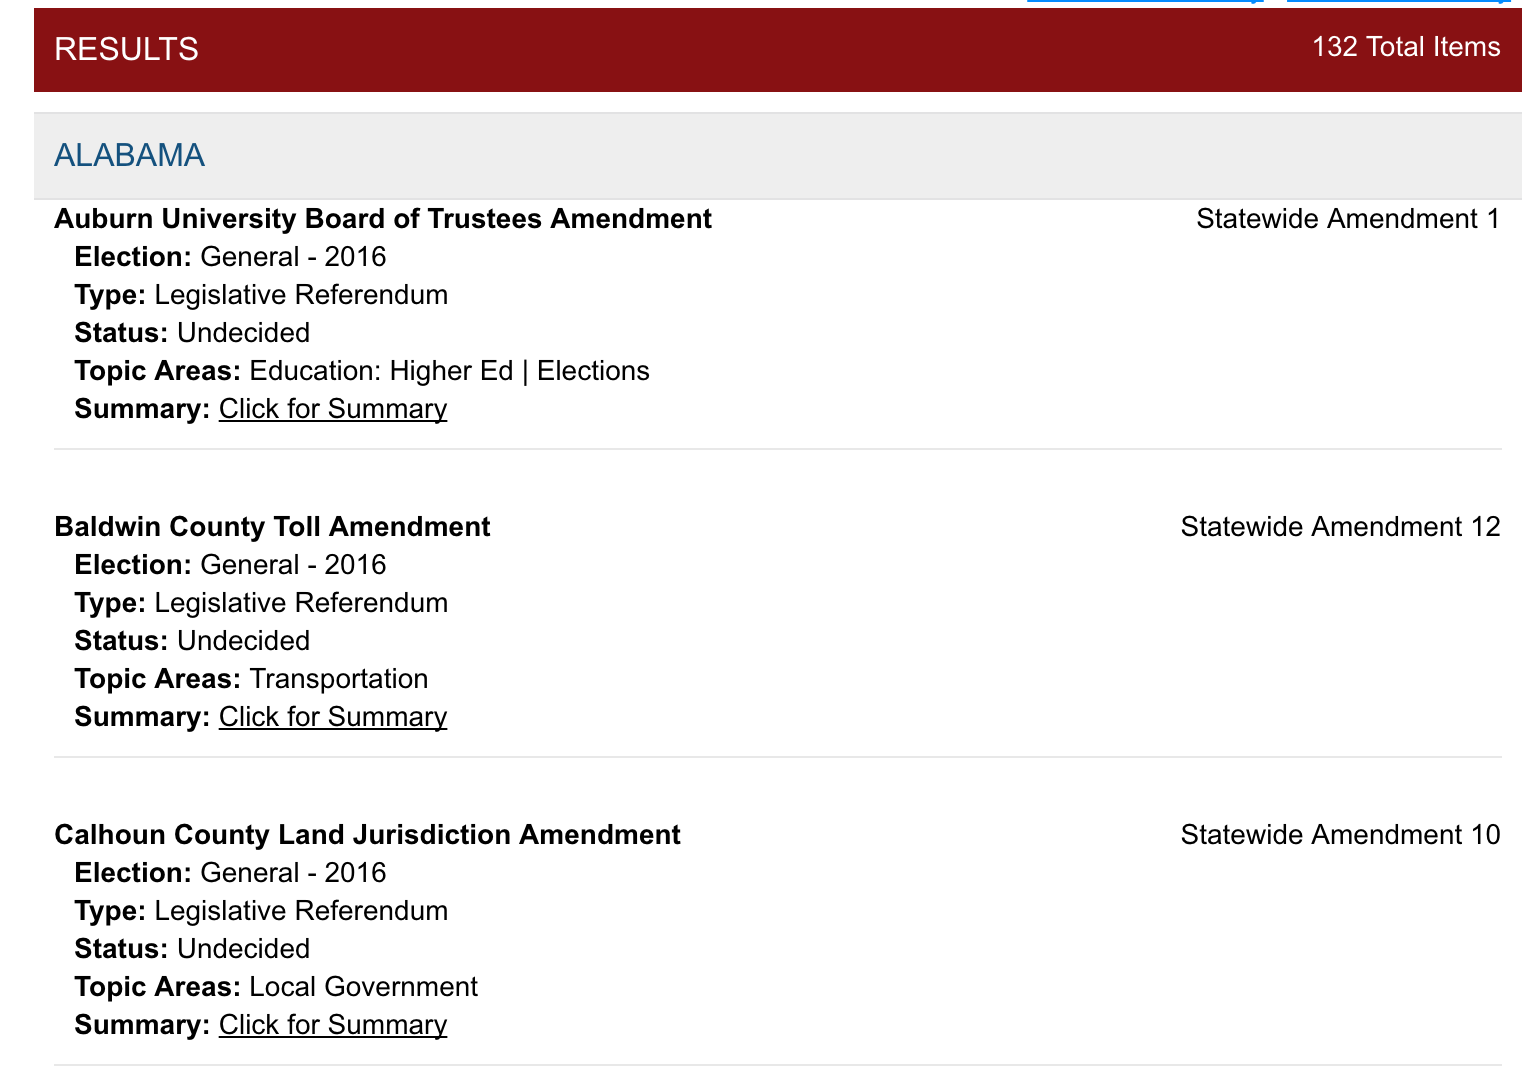
\includegraphics[width=.9\textwidth]{ncsl_results.png}\caption{Search results}
  \end{subfigure}
  \caption{Screenshots from the \href{http://www.ncsl.org/research/elections-and-campaigns/ballot-measures-database.aspx}{NCSL ballot measure database}.}\label{fig:ncsl}
\end{figure}

Say we want to know what ballot initiatives will be up for a vote in 2016 in each state. The National Conference of State Legislatures has a nice searchable database of all the initiatives sorted by year, state, and policy topic. It's available at \href{http://www.ncsl.org/research/elections-and-campaigns/ballot-measures-database.aspx}{http://www.ncsl.org/research/elections-and-campaigns/ballot-measures-database.aspx} and Figure~\ref{fig:ncsl} shows screenshots of the database. There's a lot of information here: it has the name of the ballot measure, when it's being voted on, the results, the policy topic areas it covers, and a fairly detailed summary. Unfortunately, it's not easy to download this database and it doesn't return new URL's for each search, meaning it's not easy to loop through searches automatically. 

One solution to this is to search for \textit{all} ballot measures in 2016, manually download and save the resulting HTML, then use \texttt{R} to extract the info I want. This way, I don't need to figure out how to get \texttt{R} to search for me.\footnote{This is a reasonable approach when a single search can return all the results I want. If instead we need to perform many searches, we might want to automate it. \texttt{rvest} has \texttt{html\_form()} and related functions to facilitate filling out forms on webpages. Unfortunately this package doesn't work very well in this case; instead, we'd probably need to use other, more complicated tools like the \texttt{POST()} command from the \texttt{httr} package.} 

\subsection{End Product}

I want the final result to be a spreadsheet-like object that looks something like this:~\\\\

\begin{tabular}{ccccc}
  \textbf{State} & \textbf{Name} & \textbf{Title} &  \textbf{Topic Areas} & \textbf{Summary} \\ \midrule
  Alabama & Amendment 1 & AU Board of Trustees Amendment & Education & \dots \\
  Alabama & Amendment 12 & Baldwin County Tolls & Transportation & \dots \\
  $\vdots$ & $\vdots$ & $\vdots$ & $\vdots$ & $\vdots$ \\
  Wyoming & Amendment A & Non-Permanent Fund Investment & Budgets & \dots \\\bottomrule
\end{tabular}
~\\ \\

\subsection{Selecting What We Want}

With this end goal in mind, how can we get there? First, using SelectorGadget, I can tell there are two types of tags I want to extract:
\begin{itemize}
  \item The information on ballot measures (except their state) can be extracted using this Xpath selector:\\ 
  \verb!//*[contains(concat( " ", @class, " " ), concat( " ", "divRepeaterResults", " " ))]! 
  \item States can be extracted using this Xpath selector:\\
  \verb!//*[contains(concat( " ", @class, " " ), concat( " ", "h2Headers", " " ))]!
\end{itemize}
(Don't worry about not understanding that code; I don't either.) With these selectors in hand, I can \verb!read_html()! and then select the parts of the website I want to extract using \verb!html_nodes()!. 

\begin{knitrout}
\definecolor{shadecolor}{rgb}{0.969, 0.969, 0.969}\color{fgcolor}\begin{kframe}
\begin{alltt}
\hlcom{# STEP 1, OUTSIDE OF R}
\hlcom{# Open that webpage on Chrome and search for the relevant set of ballot measures }
\hlcom{# (in this case, everything from 2016). Then download the page source.}
\hlcom{# I did this and saved it to my website.}

\hlcom{# STEP 2}
\hlcom{# Use rvest to read the html file}
\hlstd{measures} \hlkwb{=} \hlkwd{read_html}\hlstd{(}\hlstr{"http://stanford.edu/~wpmarble/webscraping_tutorial/html/ballot_measures_2016.html"}\hlstd{)}

\hlcom{# STEP 3 }
\hlcom{# Select the nodes I want -- I can use the | character to return both types of }
\hlcom{# Xpath selectors I want}
\hlstd{selector} \hlkwb{=} \hlstr{'//*[contains(concat( " ", @class, " " ), concat( " ", "divRepeaterResults", " " ))]|//*[contains(concat( " ", @class, " " ), concat( " ", "h2Headers", " " ))]'}
\hlstd{my_nodes} \hlkwb{=} \hlstd{measures} \hlopt \hlkwd{html_nodes}\hlstd{(}\hlkwc{xpath}\hlstd{=selector)}

\hlcom{# let's look at what we got}
\hlstd{my_nodes[}\hlnum{1}\hlopt{:}\hlnum{9}\hlstd{]}
\end{alltt}
\begin{verbatim}
## {xml_nodeset (9)}
## [1] <div class="h2Headers">&#13;\n            States <a id="btnClearAllS ...
## [2] <div class="h2Headers">&#13;\n            Topics<a id="btnClearAllTo ...
## [3] <div class="h2Headers">&#13;\n            Measure Type&#13;\n        ...
## [4] <div class="h2Headers">&#13;\n            Election&#13;\n        </div>
## [5] <div class="h2Headers">&#13;\n            Year&#13;\n        </div>
## [6] <div class="h2Headers">&#13;\n            Keyword Search&#13;\n      ...
## [7] <div class="h2Headers">Alabama</div>
## [8] <div class="divRepeaterResults">&#13;\n                <div class="d ...
## [9] <div class="divRepeaterResults">&#13;\n                <div class="d ...
\end{verbatim}
\begin{alltt}
\hlcom{# the first 6 nodes don't have information I want, so get rid of them}
\hlstd{my_nodes} \hlkwb{=} \hlstd{my_nodes[}\hlopt{-}\hlkwd{c}\hlstd{(}\hlnum{1}\hlopt{:}\hlnum{6}\hlstd{)]}
\end{alltt}
\end{kframe}
\end{knitrout}

\subsection{Parsing the Text Information}

The text in a node looks like this: 
\begin{Verbatim}[frame=single]
\r\n                \r\n                    State-Provided Campaign 
Finance System Funded by Imposing a Non-Resident Sales Tax\r\n            
\r\n                    Initiative 1464\r\n                
\r\n                \r\n                \r\n                
\r\n        
Election: \r\n                    General\r\n                    
-\r\n                    2016\r\n                    \r\n         
Type: \r\n                    Initiative\r\n               
\r\n                    Status: Undecided\r\n                  
Topic Areas: \r\n                     Ethics/Lobbying/Campaign Finance | 
Tax & Revenue\r\n                    \r\n        
\r\n                        Summary: Click for Summary\r\n            
\r\n                    \r\n        
Creates a campaign-finance system; allows residents to direct 
state funds to candidates; repeals the
non-resident sales-tax exemption; restricts lobbying employment by 
certain former public employees; and 
adds enforcement requirements.\r\n                \r\n              
\r\n                \r\n            
\end{Verbatim}

Here we see all the information we want, but it's all jumbled up and pasted together into one long string. But there are clearly some clues we can use to split up the string to make it more manageable. Note that the fields are separated by two line breaks, like this: \verb!\r\n \r\n! (with some extra spaces). We can split the string into chunks by using that identifier.\footnote{There is one field that isn't separated by  this double-line break, ``Topic Areas.'' I handle this below.}

\begin{knitrout}
\definecolor{shadecolor}{rgb}{0.969, 0.969, 0.969}\color{fgcolor}\begin{kframe}
\begin{alltt}
\hlstd{thetext} \hlkwb{=} \hlkwd{html_text}\hlstd{(my_nodes[[}\hlnum{128}\hlstd{]])}  \hlcom{# randomly chose 128 as an example to work thru}

\hlcom{# get rid of all those extra spaces}
\hlstd{thetext} \hlkwb{=} \hlkwd{gsub}\hlstd{(}\hlkwc{pattern} \hlstd{=} \hlstr{"[ ]+"}\hlstd{,} \hlkwc{replacement} \hlstd{=} \hlstr{" "}\hlstd{, thetext)}

\hlcom{# let's split up the string using the "\textbackslash{}r\textbackslash{}n \textbackslash{}r\textbackslash{}n" identifier plus the one field that's }
\hlcom{# not separated by two line breaks -- topic areas}
\hlstd{thetext} \hlkwb{=} \hlkwd{strsplit}\hlstd{(thetext,} \hlkwc{split}\hlstd{=} \hlstr{"\textbackslash{}r\textbackslash{}n \textbackslash{}r\textbackslash{}n|\textbackslash{}r\textbackslash{}n Topic"}\hlstd{)[[}\hlnum{1}\hlstd{]]}
\hlstd{thetext}
\end{alltt}
\begin{verbatim}
##  [1] ""                                                                                                                                                                                                                                                                                                                                                                                                                                                                                      
##  [2] " Corporate Tax Increase"                                                                                                                                                                                                                                                                                                                                                                                                                                                               
##  [3] " "                                                                                                                                                                                                                                                                                                                                                                                                                                                                                     
##  [4] " "                                                                                                                                                                                                                                                                                                                                                                                                                                                                                     
##  [5] " \r\n Election: \r\n General\r\n -\r\n 2016"                                                                                                                                                                                                                                                                                                                                                                                                                                           
##  [6] " Type: \r\n Initiative"                                                                                                                                                                                                                                                                                                                                                                                                                                                                
##  [7] " Status: Undecided"                                                                                                                                                                                                                                                                                                                                                                                                                                                                    
##  [8] " Areas: \r\n Business & Commerce | Tax & Revenue"                                                                                                                                                                                                                                                                                                                                                                                                                                      
##  [9] " \r\n Summary: Click for Summary"                                                                                                                                                                                                                                                                                                                                                                                                                                                      
## [10] " \r\n Increases annual minimum tax on corporations with Oregon sales of more than $25 million; imposes minimum tax of $30,001 plus 2.5% of amount of sales above $25 million; eliminates tax cap; benefit companies (business entities that create public benefit) taxed under current law. Applies to tax years beginning on/after January l, 2017. Revenue from tax increase goes to: public education (early childhood through grade 12); healthcare; services for senior citizens."
## [11] " "                                                                                                                                                                                                                                                                                                                                                                                                                                                                                     
## [12] " "
\end{verbatim}
\end{kframe}
\end{knitrout}

Looking better --- now we have each field on its own line, and we can get rid of the extraneous stuff to just leave what we want.

\begin{knitrout}
\definecolor{shadecolor}{rgb}{0.969, 0.969, 0.969}\color{fgcolor}\begin{kframe}
\begin{alltt}
\hlcom{# get rid of the \textbackslash{}r\textbackslash{}n,  extra whitespace, and empty entries}
\hlstd{thetext} \hlkwb{=} \hlkwd{gsub}\hlstd{(}\hlkwc{pattern}\hlstd{=}\hlstr{"\textbackslash{}\textbackslash{}r|\textbackslash{}\textbackslash{}n"}\hlstd{,} \hlkwc{replacement}\hlstd{=}\hlstr{""}\hlstd{, thetext)} \hlopt \hlstd{str_trim}
\hlstd{thetext} \hlkwb{=} \hlstd{thetext[thetext} \hlopt{!=} \hlstr{""}\hlstd{]}
\hlstd{thetext}
\end{alltt}
\begin{verbatim}
## [1] "Corporate Tax Increase"                                                                                                                                                                                                                                                                                                                                                                                                                                                          
## [2] "Election:  General - 2016"                                                                                                                                                                                                                                                                                                                                                                                                                                                       
## [3] "Type:  Initiative"                                                                                                                                                                                                                                                                                                                                                                                                                                                               
## [4] "Status: Undecided"                                                                                                                                                                                                                                                                                                                                                                                                                                                               
## [5] "Areas:  Business & Commerce | Tax & Revenue"                                                                                                                                                                                                                                                                                                                                                                                                                                     
## [6] "Summary: Click for Summary"                                                                                                                                                                                                                                                                                                                                                                                                                                                      
## [7] "Increases annual minimum tax on corporations with Oregon sales of more than $25 million; imposes minimum tax of $30,001 plus 2.5% of amount of sales above $25 million; eliminates tax cap; benefit companies (business entities that create public benefit) taxed under current law. Applies to tax years beginning on/after January l, 2017. Revenue from tax increase goes to: public education (early childhood through grade 12); healthcare; services for senior citizens."
\end{verbatim}
\end{kframe}
\end{knitrout}

Home stretch! We can easily figure out what each entry is by using the \verb!grepl()! command.

\begin{knitrout}
\definecolor{shadecolor}{rgb}{0.969, 0.969, 0.969}\color{fgcolor}\begin{kframe}
\begin{alltt}
\hlstd{title} \hlkwb{=} \hlstd{thetext[}\hlnum{1}\hlstd{]}
\hlstd{election} \hlkwb{=} \hlstd{thetext[}\hlkwd{grepl}\hlstd{(}\hlkwc{pattern} \hlstd{=} \hlstr{"^Election"}\hlstd{, thetext)]} \hlopt
  \hlkwd{gsub}\hlstd{(}\hlstr{"Election:"}\hlstd{,} \hlstr{""}\hlstd{,} \hlkwc{x} \hlstd{= .)} \hlopt \hlstd{str_trim}
\hlstd{type} \hlkwb{=} \hlstd{thetext[}\hlkwd{grepl}\hlstd{(}\hlkwc{pattern} \hlstd{=} \hlstr{"^Type"}\hlstd{, thetext)]} \hlopt
  \hlkwd{gsub}\hlstd{(}\hlstr{"Type:"}\hlstd{,} \hlstr{""}\hlstd{,} \hlkwc{x} \hlstd{= .)} \hlopt \hlstd{str_trim}
\hlstd{status} \hlkwb{=} \hlstd{thetext[}\hlkwd{grepl}\hlstd{(}\hlkwc{pattern} \hlstd{=} \hlstr{"^Status"}\hlstd{, thetext)]} \hlopt
  \hlkwd{gsub}\hlstd{(}\hlstr{"Status:"}\hlstd{,} \hlstr{""}\hlstd{,} \hlkwc{x} \hlstd{= .)} \hlopt \hlstd{str_trim}
\hlstd{topic_areas} \hlkwb{=} \hlstd{thetext[}\hlkwd{grepl}\hlstd{(}\hlkwc{pattern} \hlstd{=} \hlstr{"^Area:|Areas:"}\hlstd{, thetext)]} \hlopt
  \hlkwd{gsub}\hlstd{(}\hlstr{"Area:|Areas:"}\hlstd{,} \hlstr{""}\hlstd{,} \hlkwc{x} \hlstd{= .)} \hlopt \hlstd{str_trim}

\hlcom{# summary is a little trickier to get because the actual summary comes}
\hlcom{# the entry after the one that says "Summary: Click for Summary"}
\hlstd{summary_index} \hlkwb{=} \hlkwd{grep}\hlstd{(}\hlkwc{pattern}\hlstd{=}\hlstr{"^Summary"}\hlstd{, thetext)} \hlopt{+} \hlnum{1}
\hlstd{summary} \hlkwb{=} \hlstd{thetext[summary_index]}
\end{alltt}
\end{kframe}
\end{knitrout}

And we're done! Let's have a look:

\begin{knitrout}
\definecolor{shadecolor}{rgb}{0.969, 0.969, 0.969}\color{fgcolor}\begin{kframe}
\begin{verbatim}
## title :  Corporate Tax Increase 
## election :  General - 2016 
## type :  Initiative 
## status :  Undecided 
## summary :  Increases annual minimum tax on corporations with Oregon sales of more than $25 million; imposes minimum tax of $30,001 plus 2.5% of amount of sales above $25 million; eliminates tax cap; benefit companies (business entities that create public benefit) taxed under current law. Applies to tax years beginning on/after January l, 2017. Revenue from tax increase goes to: public education (early childhood through grade 12); healthcare; services for senior citizens. 
## topic_areas :  Business & Commerce | Tax & Revenue
\end{verbatim}
\end{kframe}
\end{knitrout}

\subsection{Scaling Up}

Now that we have the basic infrastructure in place, we can repeat this process for each node using a \verb!for! loop. The only extra thing we need to do is keep track of what state we're in. This is easy to do by first noting which indices of the nodes object contain states (i.e., those with class ``h2Headers''). Once we take care of that, we can repeat the exact same code as above and store the results in a data frame.

\begin{knitrout}
\definecolor{shadecolor}{rgb}{0.969, 0.969, 0.969}\color{fgcolor}\begin{kframe}
\begin{alltt}
\hlcom{# create state / info indicator vector}
\hlstd{state_or_info} \hlkwb{=} \hlstd{my_nodes} \hlopt \hlkwd{html_attr}\hlstd{(}\hlstr{"class"}\hlstd{)}
\hlstd{state_or_info} \hlkwb{=} \hlkwd{ifelse}\hlstd{(state_or_info} \hlopt{==} \hlstr{"h2Headers"}\hlstd{,} \hlstr{"state"}\hlstd{,} \hlstr{"info"}\hlstd{)}

\hlcom{# set up data frame to store results}
\hlstd{results_df} \hlkwb{=} \hlkwd{data.frame}\hlstd{(}\hlkwc{state} \hlstd{=} \hlkwd{rep}\hlstd{(}\hlnum{NA_character_}\hlstd{,} \hlkwd{length}\hlstd{(my_nodes)),}
                        \hlkwc{title} \hlstd{=} \hlnum{NA_character_}\hlstd{,}
                        \hlkwc{election} \hlstd{=} \hlnum{NA_character_}\hlstd{,}
                        \hlkwc{type} \hlstd{=} \hlnum{NA_character_}\hlstd{,}
                        \hlkwc{status} \hlstd{=} \hlnum{NA_character_}\hlstd{,}
                        \hlkwc{topic_areas} \hlstd{=} \hlnum{NA}\hlstd{,}
                        \hlkwc{summary} \hlstd{=} \hlnum{NA_character_}\hlstd{,}
                        \hlkwc{stringsAsFactors} \hlstd{= F)}


\hlstd{state} \hlkwb{=} \hlnum{NA_character_} \hlcom{# this variable will keep track of what state we're in}

\hlcom{# loop through all the nodes}
\hlkwa{for} \hlstd{(i} \hlkwa{in} \hlnum{1}\hlopt{:}\hlkwd{length}\hlstd{(my_nodes))\{}

  \hlcom{# first see if the node tells us what state we're in; if so, update}
  \hlcom{# the state variable}
  \hlkwa{if} \hlstd{(state_or_info[i]} \hlopt{==} \hlstr{"state"}\hlstd{) \{}
    \hlstd{state} \hlkwb{=} \hlkwd{html_text}\hlstd{(my_nodes[[i]])}
  \hlstd{\}}

  \hlcom{# if it doesn't say what state we're in, apply the parsing code from above}
  \hlkwa{else} \hlstd{\{}
    \hlstd{results_df}\hlopt{$}\hlstd{state[i]} \hlkwb{=} \hlstd{state} \hlcom{# fill in state}

    \hlcom{# parse text like above}
    \hlstd{thetext} \hlkwb{=} \hlkwd{html_text}\hlstd{(my_nodes[[i]])}
    \hlstd{thetext} \hlkwb{=} \hlkwd{gsub}\hlstd{(}\hlkwc{pattern} \hlstd{=} \hlstr{"[ ]+"}\hlstd{,} \hlkwc{replacement} \hlstd{=} \hlstr{" "}\hlstd{, thetext)}
    \hlstd{thetext} \hlkwb{=} \hlkwd{strsplit}\hlstd{(thetext,} \hlkwc{split}\hlstd{=} \hlstr{"\textbackslash{}r\textbackslash{}n \textbackslash{}r\textbackslash{}n|\textbackslash{}r\textbackslash{}n Topic"}\hlstd{)[[}\hlnum{1}\hlstd{]]}

    \hlstd{thetext} \hlkwb{=} \hlkwd{gsub}\hlstd{(}\hlkwc{pattern}\hlstd{=}\hlstr{"\textbackslash{}\textbackslash{}r|\textbackslash{}\textbackslash{}n"}\hlstd{,} \hlkwc{replacement}\hlstd{=}\hlstr{""}\hlstd{, thetext)} \hlopt \hlstd{str_trim}
    \hlstd{thetext} \hlkwb{=} \hlstd{thetext[thetext} \hlopt{!=} \hlstr{""}\hlstd{]}


    \hlstd{results_df}\hlopt{$}\hlstd{title[i]} \hlkwb{=} \hlstd{thetext[}\hlnum{1}\hlstd{]}
    \hlstd{results_df}\hlopt{$}\hlstd{election[i]} \hlkwb{=} \hlstd{thetext[}\hlkwd{grepl}\hlstd{(}\hlkwc{pattern} \hlstd{=} \hlstr{"^Election"}\hlstd{, thetext)]} \hlopt
      \hlkwd{gsub}\hlstd{(}\hlstr{"Election:"}\hlstd{,} \hlstr{""}\hlstd{,} \hlkwc{x} \hlstd{= .)} \hlopt \hlstd{str_trim}
    \hlstd{results_df}\hlopt{$}\hlstd{type[i]} \hlkwb{=} \hlstd{thetext[}\hlkwd{grepl}\hlstd{(}\hlkwc{pattern} \hlstd{=} \hlstr{"^Type"}\hlstd{, thetext)]} \hlopt
      \hlkwd{gsub}\hlstd{(}\hlstr{"Type:"}\hlstd{,} \hlstr{""}\hlstd{,} \hlkwc{x} \hlstd{= .)} \hlopt \hlstd{str_trim}
    \hlstd{results_df}\hlopt{$}\hlstd{status[i]} \hlkwb{=} \hlstd{thetext[}\hlkwd{grepl}\hlstd{(}\hlkwc{pattern} \hlstd{=} \hlstr{"^Status"}\hlstd{, thetext)]} \hlopt
      \hlkwd{gsub}\hlstd{(}\hlstr{"Status:"}\hlstd{,} \hlstr{""}\hlstd{,} \hlkwc{x} \hlstd{= .)} \hlopt \hlstd{str_trim}
    \hlstd{results_df}\hlopt{$}\hlstd{topic_areas[i]} \hlkwb{=} \hlstd{thetext[}\hlkwd{grepl}\hlstd{(}\hlkwc{pattern} \hlstd{=} \hlstr{"^Area:|Areas:"}\hlstd{, thetext)]} \hlopt
      \hlkwd{gsub}\hlstd{(}\hlstr{"Area:|Areas:"}\hlstd{,} \hlstr{""}\hlstd{,} \hlkwc{x} \hlstd{= .)} \hlopt \hlstd{str_trim}

    \hlstd{summary_index} \hlkwb{=} \hlkwd{grep}\hlstd{(}\hlkwc{pattern}\hlstd{=}\hlstr{"^Summary"}\hlstd{, thetext)} \hlopt{+} \hlnum{1}
    \hlstd{results_df}\hlopt{$}\hlstd{summary[i]} \hlkwb{=} \hlstd{thetext[summary_index]}
  \hlstd{\}}
\hlstd{\}}
\hlstd{results_df} \hlkwb{=} \hlstd{results_df[}\hlopt{!}\hlkwd{is.na}\hlstd{(results_df}\hlopt{$}\hlstd{state),]}

\hlcom{# let's have a look at a bit of the final product (some variables omitted for space)}
\hlkwd{print}\hlstd{(results_df[}\hlnum{1}\hlopt{:}\hlnum{5}\hlstd{,} \hlnum{1}\hlopt{:}\hlnum{3}\hlstd{],} \hlkwc{row.names} \hlstd{= F)}
\end{alltt}
\begin{verbatim}
##    state                                         title       election
##  Alabama Auburn University Board of Trustees Amendment General - 2016
##  Alabama                 Baldwin County Toll Amendment General - 2016
##  Alabama    Calhoun County Land Jurisdiction Amendment General - 2016
##  Alabama       County Affairs Administration Amendment General - 2016
##  Alabama                         Impeachment Amendment General - 2016
\end{verbatim}
\end{kframe}
\end{knitrout}

And voil\`{a}! We took the data from a mess of HTML and turned it into a nice, spreadsheet-like database that is ready to be used in our analysis. 

\section{A Very, Very Short Introduction to APIs}

A much easier way to download data from websites is through an application programming interface. The idea behind an API is that you send a request to the server using a precisely defined query structure, and the server sends you the data you asked for in a precisely defined format. 

With most APIs, you just need to know how to format the URL, and there is documentation telling you what to include. For example, the OMDb API lets you download the IMDb data for any movie or TV show by going to a URL like this: \verb!http://omdbapi.com/?parameter1=value1&parameter2=value2!. The parameter ``t'' is for title, so if I want to look up information about ``Game of Thrones,'' I can follow this link: \href{http://omdbapi.com/?t=game+of+thrones}{http://omdbapi.com/?t=game+of+thrones}. (Other possible parameters can be found in the \href{http://www.omdbapi.com/}{OMDb documentation}.) 

You'll notice that the information is returned in JSON, which is a data storage format that's often used on websites. We'll have to convert this to an \texttt{R} format. So how can we automate webscraping using an API? We'll again use \texttt{rvest} and then process the JSON using the package \texttt{rjson}.

As a small example, let's look up all the TV shows in the past 10 years that got Emmy nominations for best drama and compare their IMDb ratings. 

\begin{knitrout}
\definecolor{shadecolor}{rgb}{0.969, 0.969, 0.969}\color{fgcolor}\begin{kframe}
\begin{alltt}
\hlcom{# install rjson}
\hlkwa{if} \hlstd{(}\hlopt{!}\hlkwd{require}\hlstd{(rjson)) \{}\hlkwd{install.packages}\hlstd{(}\hlstr{"rjson"}\hlstd{);}\hlkwd{library}\hlstd{(rjson)\}}
\end{alltt}
\end{kframe}
\end{knitrout}

\begin{knitrout}
\definecolor{shadecolor}{rgb}{0.969, 0.969, 0.969}\color{fgcolor}\begin{kframe}
\begin{alltt}
\hlstd{list_of_shows} \hlkwb{=} \hlkwd{c}\hlstd{(}\hlstr{"breaking bad"}\hlstd{,} \hlstr{"mad men"}\hlstd{,} \hlstr{"game of thrones"}\hlstd{,}
                  \hlstr{"homeland"}\hlstd{,} \hlstr{"house of cards"}\hlstd{,} \hlstr{"true detective"}\hlstd{,}
                  \hlstr{"orange is the new black"}\hlstd{,} \hlstr{"the americans"}\hlstd{,} \hlstr{"mr robot"}\hlstd{,}
                  \hlstr{"boardwalk empire"}\hlstd{,} \hlstr{"the good wife"}\hlstd{,} \hlstr{"dexter"}\hlstd{,}
                  \hlstr{"lost"}\hlstd{,} \hlstr{"true blood"}\hlstd{,} \hlstr{"house"}\hlstd{,} \hlstr{"big love"}\hlstd{,} \hlstr{"downton abbey"}\hlstd{,}
                  \hlstr{"damages"}\hlstd{,} \hlstr{"boston legal"}\hlstd{,} \hlstr{"grey's anatomy"}\hlstd{,} \hlstr{"the sopranos"}\hlstd{,}
                  \hlstr{"heroes"}\hlstd{,} \hlstr{"better call saul"}\hlstd{)}

\hlstd{show_db} \hlkwb{=} \hlkwd{data.frame}\hlstd{(}\hlkwc{title} \hlstd{= list_of_shows,}
                     \hlkwc{year} \hlstd{=} \hlnum{NA}\hlstd{,} \hlkwc{genre} \hlstd{=} \hlnum{NA}\hlstd{,} \hlkwc{plot} \hlstd{=} \hlnum{NA}\hlstd{,} \hlkwc{country} \hlstd{=} \hlnum{NA}\hlstd{,}
                     \hlkwc{awards} \hlstd{=} \hlnum{NA}\hlstd{,} \hlkwc{metascore} \hlstd{=} \hlnum{NA}\hlstd{,} \hlkwc{imdbrating} \hlstd{=} \hlnum{NA}\hlstd{,}
                     \hlkwc{imdbvotes} \hlstd{=} \hlnum{NA}\hlstd{,} \hlkwc{imdbid} \hlstd{=} \hlnum{NA}\hlstd{,} \hlkwc{totalseasons} \hlstd{=} \hlnum{NA}\hlstd{)}

\hlcom{# construct the url for each show by pasting the name of the show after}
\hlcom{# the API base, and encoding using URLencode(). }
\hlkwa{for} \hlstd{(show} \hlkwa{in} \hlstd{list_of_shows)\{}
  \hlstd{show_url} \hlkwb{=} \hlkwd{paste0}\hlstd{(}\hlstr{"http://omdbapi.com/?&t="}\hlstd{,} \hlkwd{URLencode}\hlstd{(show,} \hlkwc{reserved} \hlstd{= T))}
  \hlstd{show_info} \hlkwb{=} \hlkwd{read_html}\hlstd{(show_url)} \hlopt \hlstd{html_text} \hlopt \hlstd{fromJSON}

  \hlstd{show_db}\hlopt{$}\hlstd{year[show_db}\hlopt{$}\hlstd{title}\hlopt{==}\hlstd{show]} \hlkwb{=} \hlstd{show_info}\hlopt{$}\hlstd{Year}
  \hlstd{show_db}\hlopt{$}\hlstd{genre[show_db}\hlopt{$}\hlstd{title}\hlopt{==}\hlstd{show]} \hlkwb{=} \hlstd{show_info}\hlopt{$}\hlstd{Genre}
  \hlstd{show_db}\hlopt{$}\hlstd{plot[show_db}\hlopt{$}\hlstd{title}\hlopt{==}\hlstd{show]} \hlkwb{=} \hlstd{show_info}\hlopt{$}\hlstd{Plot}
  \hlstd{show_db}\hlopt{$}\hlstd{country[show_db}\hlopt{$}\hlstd{title}\hlopt{==}\hlstd{show]} \hlkwb{=} \hlstd{show_info}\hlopt{$}\hlstd{Country}
  \hlstd{show_db}\hlopt{$}\hlstd{awards[show_db}\hlopt{$}\hlstd{title}\hlopt{==}\hlstd{show]} \hlkwb{=} \hlstd{show_info}\hlopt{$}\hlstd{Awards}
  \hlstd{show_db}\hlopt{$}\hlstd{metascore[show_db}\hlopt{$}\hlstd{title}\hlopt{==}\hlstd{show]} \hlkwb{=} \hlstd{show_info}\hlopt{$}\hlstd{Metascore}
  \hlstd{show_db}\hlopt{$}\hlstd{imdbrating[show_db}\hlopt{$}\hlstd{title}\hlopt{==}\hlstd{show]} \hlkwb{=} \hlstd{show_info}\hlopt{$}\hlstd{imdbRating}
  \hlstd{show_db}\hlopt{$}\hlstd{imdbvotes[show_db}\hlopt{$}\hlstd{title}\hlopt{==}\hlstd{show]} \hlkwb{=} \hlstd{show_info}\hlopt{$}\hlstd{imdbVotes}
  \hlstd{show_db}\hlopt{$}\hlstd{imdbid[show_db}\hlopt{$}\hlstd{title}\hlopt{==}\hlstd{show]} \hlkwb{=} \hlstd{show_info}\hlopt{$}\hlstd{imdbID}
  \hlstd{show_db}\hlopt{$}\hlstd{totalseasons[show_db}\hlopt{$}\hlstd{title}\hlopt{==}\hlstd{show]} \hlkwb{=} \hlstd{show_info}\hlopt{$}\hlstd{totalSeasons}
\hlstd{\}}
\hlstd{show_db[}\hlnum{1}\hlopt{:}\hlnum{5}\hlstd{,} \hlkwd{c}\hlstd{(}\hlnum{1}\hlopt{:}\hlnum{3}\hlstd{,} \hlnum{8}\hlstd{)]}
\end{alltt}
\begin{verbatim}
##             title      year                     genre imdbrating
## 1    breaking bad 2008–2013    Crime, Drama, Thriller        9.5
## 2         mad men 2007–2015                     Drama        8.6
## 3 game of thrones     2011– Adventure, Drama, Fantasy        9.5
## 4        homeland     2011–     Crime, Drama, Mystery        8.4
## 5  house of cards     2013–                     Drama        9.0
\end{verbatim}
\end{kframe}
\end{knitrout}

Now again, we have a data frame that's amenable to analysis, like Figure~\ref{fig:tvshows}. There's a lot more to learn about APIs, so I encourage you to explore more --- but many will follow this basic formula: base URL + ? + parameters. 

\begin{knitrout}
\definecolor{shadecolor}{rgb}{0.969, 0.969, 0.969}\color{fgcolor}\begin{figure}

{\centering 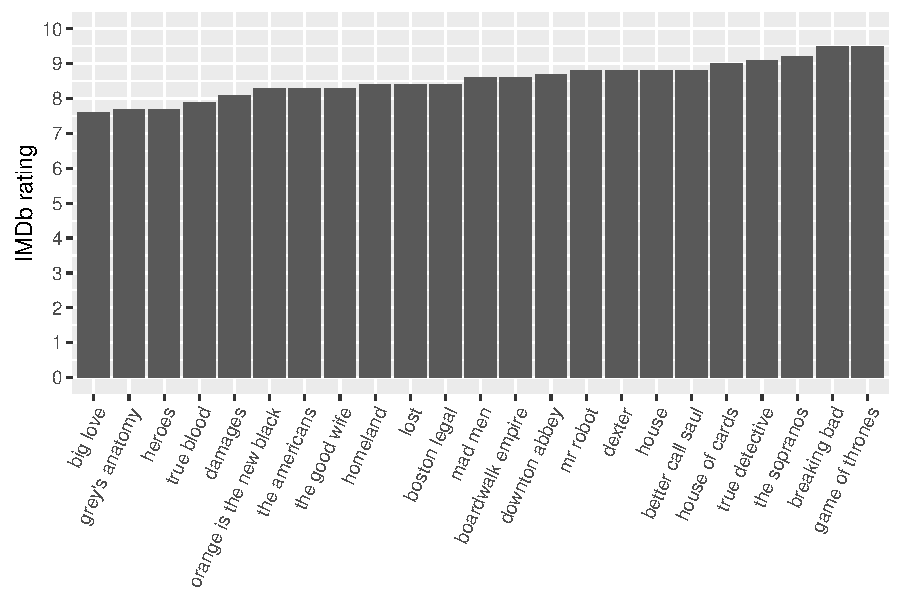
\includegraphics[width=\maxwidth]{figure/tvshows-1} 

}

\caption[IMDb ratings of Best Drama-nominated TV shows, 2006-2016]{IMDb ratings of Best Drama-nominated TV shows, 2006-2016.}\label{fig:tvshows}
\end{figure}


\end{knitrout}


\bibliographystyle{apsr}
\bibliography{/Users/Will/Dropbox/master_bib_file/library.bib}

\end{document}
